%%%%%%%%%%%%%%%%%%%%%%%%%%%%%%%%%%%%%%%%%%%%%%%%%%%%%%%%%%%%%%%%%%%%%%
% LaTeX Example: Project Report
%
% Source: http://www.howtotex.com
%
% Feel free to distribute this example, but please keep the referral
% to howtotex.com
% Date: March 2011 
% 
%%%%%%%%%%%%%%%%%%%%%%%%%%%%%%%%%%%%%%%%%%%%%%%%%%%%%%%%%%%%%%%%%%%%%%
% How to use writeLaTeX: 
%
% You edit the source code here on the left, and the preview on the
% right shows you the result within a few seconds.
%
% Bookmark this page and share the URL with your co-authors. They can
% edit at the same time!
%
% You can upload figures, bibliographies, custom classes and
% styles using the files menu.
%
% If you're new to LaTeX, the wikibook is a great place to start:
% http://en.wikibooks.org/wiki/LaTeX
%
%%%%%%%%%%%%%%%%%%%%%%%%%%%%%%%%%%%%%%%%%%%%%%%%%%%%%%%%%%%%%%%%%%%%%%
% Edit the title below to update the display in My Documents
%\title{Project Report}
%
%%% Preamble
\documentclass[paper=a4, fontsize=11pt]{scrartcl}
\usepackage[T1]{fontenc}
\usepackage{fourier}
\usepackage[english]{babel}			 % English language/hyphenation												
\usepackage[protrusion=true,expansion=true]{microtype}	
\usepackage{amsmath,amsfonts,amsthm} % Math packages
\usepackage[pdftex]{graphicx}	
\usepackage{url}

\usepackage{sectsty}   %%% Custom sectioning
\allsectionsfont{\centering \normalfont\scshape}


%%% Custom headers/footers (fancyhdr package)
\usepackage{fancyhdr}
\pagestyle{fancyplain}
\fancyhead{}											% No page header
\fancyfoot[L]{}											% Empty 
\fancyfoot[C]{}											% Empty
\fancyfoot[R]{\thepage}									% Pagenumbering
\renewcommand{\headrulewidth}{0pt}			% Remove header underlines
\renewcommand{\footrulewidth}{0pt}				% Remove footer underlines
\setlength{\headheight}{13.6pt}


%%% Equation and float numbering
\numberwithin{equation}{section}		% Equationnumbering: section.eq#
\numberwithin{figure}{section}			% Figurenumbering: section.fig#
\numberwithin{table}{section}				% Tablenumbering: section.tab#


%%% Maketitle metadata
\newcommand{\horrule}[1]{\rule{\linewidth}{#1}} 	% Horizontal rule

\title{
		%\vspace{-1in} 	
		\usefont{OT1}{bch}{b}{n}
		\normalfont \normalsize \textsc{School of Computer Science} \\ 
        \normalsize \textsc{High Performance Architecture (COMPSCI 243)} \\
        [25pt]
		\horrule{0.5pt} \\[0.4cm]
		\huge GPU Benchmarking Report \\
		\horrule{2pt} \\[0.5cm]
}
\author{
		\normalfont 								
        \normalsize
        Zahra Montazeri (84168407) \\[-3pt]		
        \normalsize 
        \newline
        \normalsize
        Nitin Agarwal (84246130) \\[-3pt]		
        \normalsize 
        \newline
        \newline
        \today
}
\date{}
\newpage

%%% Begin document
\begin{document}
\maketitle
\newpage
\tableofcontents
\newpage
\section{Vision and Scope}
In this project, a set of well-defined test cases for GPU have been used to compare the performances of different graphics cards across differnt platforms. The main focus of the project has been to use the various test cases with similar settings on multiple graphics cards, keeping everything else the same. We perform benchmarking on three different NVIDIA Graphic Cards and profile the test cases using an NVIDIA profiler \textbf{nvprof}. We show the results of each of the test cases and further perform analysis.\\

The project involved searching of well-known, published test cases, which could be tested on Linux platforms. All benchmarks have been performed using the release 3.1 version of the Rodinia \ref{•}. Several test cases from Rodinia were profiled using nvprof (NVIDIA profiling tool), which is a command-line profiler available for Linux, Windows, and OS X. It helps users to understand and optimize the performance of cuda applications and easily compare and analyze the result of benchmarks on different GPUs. A cuda version of 7.5 was used to benchmark all three graphic cards in this project. The three NVIDIA graphics cards benchmarked are GTX 630, GTX 650 \& Quadro M6000.\\

We chose seven different test cases and profiled several parameters for each test case. We compare and analyze these values across all three different GPU cards. We profiled the following parameters:

\begin{itemize}
\item
\textit{Total time for all API calls: } We added up the duration of all API calls together to get the total amount of time spending by API calls. 

\item
\textit{Total time for all Kernel calls: } We added up the duration of all kernel calls together to get the total amount of time spending by kernel calls. 

\item
\textit{Number of registers per thread for each Kernel call: } The number of registers in use affects the occupancy of your GPU since the total number of registers per multiprocessor is limited. In fact it's dependant on the problem but we will want to have our occupancy as high as possible, to avoid ressources from being wasted. On the other hand it is possible that the code is slowed down if the number of registers is restricted.

\item
\textit{Temperature: } We understand that temperature and fan-speed would be more relevant in for benchmarking mobile GPU's, but for completeness we profiled them both.

\item
\textit{Fan Speed: All the graphics cards requires a robust fan to keep it from overheating under a load. This parameter is the percentage of the total amount of fan power depending on how much you tax the graphics card in the system. You may want to adjust its fan speed to provide better cooling or produce less noise when not pushing it to its limits.}
\end{itemize}



\newpage
\section{Description of Benchmarks}
This section provides a brief description of all the seven test cases used 
to benchmark the three NVIDIA GPU cards.

\subsection{Breadth First Search}
Graph algorithms are fundamental and widely used in many disciplines and application areas. Large graphs involving millions of vertices are common in scientific and engineering applications. This benchmark suite provides the GPU implementations of breadth-first search (BFS) algorithm which traverses all the connected components in a graph.

\subsection{K-Nearest Neighbor}
NN (Nearest Neighbor) finds the k-nearest neighbors from an unstructured data set. The sequential NN algorithm reads in one record at a time, calculates the Euclidean distance from the target latitude and longitude, and evaluates the k nearest neighbors. The parallel versions read in many records at a time, execute the distance calculation on multiple threads, and the master thread updates the list of nearest neighbors.

\subsection{B+Tree}
B+ Tree application has many internal commands that maintain database and process querries. Only J and K commands had enough parallelism to be ported to parallel languages (OpenMP, CUDA, OpenCL). In these implementations, in case of both J and K, the same algorithms (optimized for exposing fine-grained parallelism) were used for fair comparison purposes. For C/OpenMP execution, it is possible to use the original algorithm.

\subsection{PathFinder}
PathFinder uses dynamic programming to find a path on a 2-D grid from the bottom row to the top row with the smallest accumulated weights, where each step of the path moves straight ahead or diagonally ahead. It iterates row by row, each node picks a neighboring node in the previous row that has the smallest accu- mulated weight, and adds its own weight to the sum.
This kernel uses the technique of ghost zone optimization.

\subsection{LU Decomposition}
LU Decomposition is an algorithm to calculate the solutions of a set of linear equations. The LUD kernel decomposes a matrix as the product of a lower triangular matrix and an upper triangular matrix.

\subsection{Gaussian Elimination}
Gaussian Elimination computes result row by row, solving for all of the variables in a linear system. The algorithm must synchronize between iterations, but the values calculated in each iteration can be computed in parallel.

\subsection{hotspot}
HotSpot is a widely used tool to estimate processor temperature based on an architectural floorplan and simulated power measurements. The thermal simulation iteratively solves a series of differential equations for block. Each output cell in the computational grid represents the average temperature value of the corresponding area of the chip. Our CUDA implementation re-implements the transient thermal differential equation solver from HotSpot.






\newpage
\section{Methodology}
The main objective of this project is to use same test cases, with similar settings on three different NVIDIA GPU graphics cards. During benchmarking of the seven test cases, we made sure that no other programs, code etc were running on these three machines. We further ensured that all the settings were as similar as possible e.g for GPU architecture, cuda settings etc.\\


Instead of profiling the total execution time, which collectively sums up the CPU \& GPU running time, we only profiled the time for all the API calls and the Kernel calls. Since we are only concerned with GPU benchmarking, this seems reasonable as all three machines have different processors (Table \ref{table1}), which would lead to different CPU running times. We also profiled the number of registers used per thread for each kernel call in each program. And lastly we profiled the GPU temperature and fan speed. Though we understand that for desktop machine people are not that concerned about them, however when compiling different servers temperature and fan speed play an important role.  

\subsection{GPU Parallelisation}
The GPU computing approach uses graphic card to perform the calculation in parallel. This approach is based on CUDA which is made by NVIDIA and works on NVIDIA graphic cards that have Compute Capability 2.0 or higher. The point is worth mentioning that only hydrodynamic calculations are performed on the GPU and the additional calculations are run on the CPU. Then these calculations are parallelised using shared memory approach, OpenMP.

\subsection{Hardware}
The following are the specifications of the three NVIDIA graphic cards which were used to perform benchmark:

\begin{table}[!h]
\caption{GPU specifications}
\centering
\begin{tabular}{|l| c| c| c|}
	\hline
	GPU & Compute Capability & Number of CUDA cores & Memory (GB)\\
	\hline
    GeForce GT 630 & 2.1 & 96 & 1.8  \\
	\hline
    Geforce GTX 650 & 3.0 & 384 & 5 \\
	\hline
    Quadro 6000 & 2.0 & 448 & 6 \\
	\hline
\end{tabular}
\label{table1}
\end{table}

The specifications of the machines in which the graphic cards resided are shown in the below table:

\begin{table}[!h]
\caption{Hardware Platforms}
\centering
\begin{tabular}{| c| c| c| c|}
	\hline
	  & Processor & Memory (GB)& Operating system\\
	\hline
    1  & Intel Xeon(R) E5405 (4 cores, 2.00GHz) & 2& ubuntu 14.04 \\
	\hline
    2  & Nitincomp?? & 16 & ubuntu 14.04 \\
	\hline
    3  & Intel Core 2 Quad Q9400 (4 cores, 2.66GHz) & 7.8& ubuntu 14.04 \\
	\hline
\end{tabular}
\label{table2}
\end{table}

\newpage
\clearpage
\subsection{Software}
All benchmarks have been performed using the release 3.1 version of the Rodinia: accelerating Compute-Intensive Applications with Accelerators. It released to address some concerns in  which platforms face. For example, there are many suites for parallel computing on general-purpose CPU architectures, but accelerators fall into a gap that is not covered by previous benchmark development.

\newpage
\clearpage
\section{Comparison of the Graphic Cards}
Here we have the comparison in performance among GTX 650, GT 630 and Quadro 600 based on reported evaluations. Later we will compare this evaluation with our results to show how they match with the expected values. 

\subsection{Overal evaluation}
We have used overal evaluations for the aforementioned graphics cards reported by Game Debate. Following is a brief explanation of each parameter in Table \ref{GPU comparison}. Performance score reflects how well you feel the hardware meets your expectations on performance. Lifespan score reflects how long you feel this hardware will last and perform its function. Value score represents how well the graphics card is placed with regards to its price to performance. 

\begin{table}[!h]
\caption{Evaluation published by Game Debate}
\centering
\begin{tabular}{|l|c|c|c|}
	\hline
	 & Geforce GTX 650 & Quadro 6000 & Geforce GT 630\\
	\hline
      	GPU Architechture & 1 & 1.3 & 1 \\
	\hline
    	GPU Memory & 0.5 & 1 & 0.3 \\
	\hline
    	GPU Display & 0.4 & 0.8 & 0.2\\
	\hline
	GPU Outputs & 1 & 0.7 & 1 \\
	\hline
	GPU Features & 1 & 1.3 & 1 \\
	\hline

\end{tabular}
\label{GPU comparison}
\end{table}

A more detailed explanation:\\
The GTX 650 has a 484 MHz higher core clock speed but 24 fewer Texture Mapping Units than the Quadro 6000. The lower TMU count doesn't matter, though, as altogether the GTX 650 manages to provide 1.8 GTexel/s better texturing performance. This still holds weight but shader performance is generally more relevant, particularly since both of these GPUs support at least DirectX 10.The GTX 650 has a 248 MHz higher core clock speed and 16 more Texture Mapping Units than the GeForce GT 630. This results GT 630 performs worse than the other two.

The GTX 650 has a 484 MHz higher core clock speed than the Quadro 6000, but the Quadro 6000 has 32 more Render Output Units than the GTX 650. As a result, the Quadro 6000 exhibits a 10.7 GPixel/s better Pixel Fill Rate than the GTX 650. However, both GPUs support DirectX 9 or above, and pixeling performance is only really relevant when comparing older cards. These two graphics cards have higher core clock speed and more Render Output Units than the GeForce GT 630. This results GT 630 again to perform the worst.

The GTX 650 was released over a year more recently than the Quadro 6000, and so the GTX 650 is likely to have better driver support, meaning it will be more optimized for running the latest games when compared to the Quadro 6000.The GTX 650 was released less than a year after the GeForce GT 630, and so they are likely to have similar driver support for optimizing performance when running the latest games. 

The Quadro 6000 has 4096 MB more video memory than the GTX 650, so is likely to be much better at displaying game textures at higher resolutions. This is supported by the fact that the Quadro 6000 also has superior memory performance overall. The GeForce GTX 650 1GB and the GeForce GT 630 have the same amount of video memory, but are likely to provide slightly different experiences when displaying game textures at high resolutions.

The Quadro 6000 has 63.4 GB/sec greater memory bandwidth than the GTX 650, which means that the memory performance of the Quadro 6000 is much better than the GTX 650. These two have greater memory bandwidth than the GeForce GT 630, which means that the memory performance of the GTX 630 is much worse than the other two. 

The GeForce GTX 650 2GB has 384 Shader Processing Units, the Quadro 6000 has 448 and the GeForce GT 630 has 96. However, the actual shader performance of the GTX 650 is 406, the actual shader performance of the Quadro 6000 is 514 and the actual shader performance of the GeForce GT 630 is 156. The Quadro 6000 having 108 better shader performance and an altogether better performance when taking into account other relevant data means that the Quadro 6000 delivers a significantly smoother and more efficient experience when processing graphical data than the GTX 650 and GT 630. 

The GTX 650 transistor size technology is 12 nm (nanometers) smaller than the Quadro 6000 as well as GT 630. This means that the GTX 650 is expected to run slightly cooler and achieve higher clock frequencies than both the Quadro 6000 and GT 630.

The GeForce GTX 650 2GB requires 64 Watts to run, the GeForce GT 630 requires 65 Watts and the Quadro 6000 requires 204 Watts. We would recommend a PSU with at least 400 Watts for the GTX 650 and a PSU with at least 600 Watts for the Quadro 6000. The Quadro 6000 requires 140 Watts more than the GTX 650 to run. The difference is significant enough that the Quadro 6000 may have an adverse affect on your yearly electricity bills in comparison to the GTX 650. The GeForce GT 630 requires 1 Watts more than the GTX 650 to run. The difference is not significant enough for the GeForce GT 630 to have a noticeably larger impact on your yearly electricity bills than the GTX 650.

In terms of overall gaming performance, the graphical capabilities of the Nvidia Quadro 6000 are noticeably better than the Nvidia GeForce GTX 650 2GB and massively better than the GT 630.

Here we also have user evaluation on the same graphics cards published by Game Debate.

\begin{table}[!h]
\caption{User evaluation }
\centering
\begin{tabular}{|l|c|c|c|}
	\hline
	& Geforce GT 630 & Geforce GTX 650 & Quadro 6000 \\
	\hline
      Performance & 6.0 & 8.5 & 9.4 \\
	\hline
    Life Span & 7.3 & 8.5 & 7.9 \\
	\hline
    Value & 6.9 & 8.7 & 5.4\\
	\hline
	Overall & 7.0 & 8.6 & 7.4 \\
	\hline

\end{tabular}
\label{User evaluation}
\end{table}

Now, let's have a brief description of the three graphics cards we used.

\subsection {Review on GT 630}
GeForce GT 630 is Middle-Class Graphics Card based on the first revision of the Fermi Architecture. The Fermi Architecture is manufactured with a 40nm technology and uses a technique known as Hot Clocking: The Shaders are clocked twice as fast as the Central Unit. While this leads to a reasonable performance boost, it causes enormous amounts of energy dissipation, leading, ultimately, to a significantly higher operating temperature.
Fermi is also the first GPU architecture with fully cached memory access which increases memory performance. 

\subsection{Review on GTX 650}
GeForce GTX 650 2GB is a fast-middle-class GPU part of the 600 Series released by NVIDIA in 2012.
This version features a frame buffer of 2GB. It's known that this GPU does not benefit in any way from a 2GB frame buffer and so this GPU's performance is on level with the 1GB variant. Check the page of the 1GB version for more information about but please note this GPU is just a fast GT 640, paired with GDDR5. Its performance is nothing like next in series - GeForce GTX 650 Ti and barely any fast than previous GTX 550 Ti.

\subsection{Review on Quadro 6000}
Quadro 6000 is a high-end professional card based on the 40nm, Fermi architecture. It's based on the Fermi GF100 GPU and thus offers 448 Shader Processing Units, 56 TMUs and 48 ROPs, on a 384-bit memory interface of fast GDDR5. The central unit runs at 574MHz and the memory clock operates at up to 747MHz. It has a L2 Cache of 768KB and a rated board TDP of 204 Watts. 
Despite exhibiting similarities to GeForce GTX 470, due to being under-clocked and because Quadro 6000's drivers are only certified for professional applications only, its gaming performance is up to 10 persent slower than GeForce GTX 470.

\newpage
\section{Benchmarking using a GeForce GT 630}
These tests have been performed using a GeForce GT 630 and hardware platform 1 specified in Table \ref{table2}. The below figures depict the time take for each individual API call for all seven test cases.

\begin{figure*}[!h]
\centering
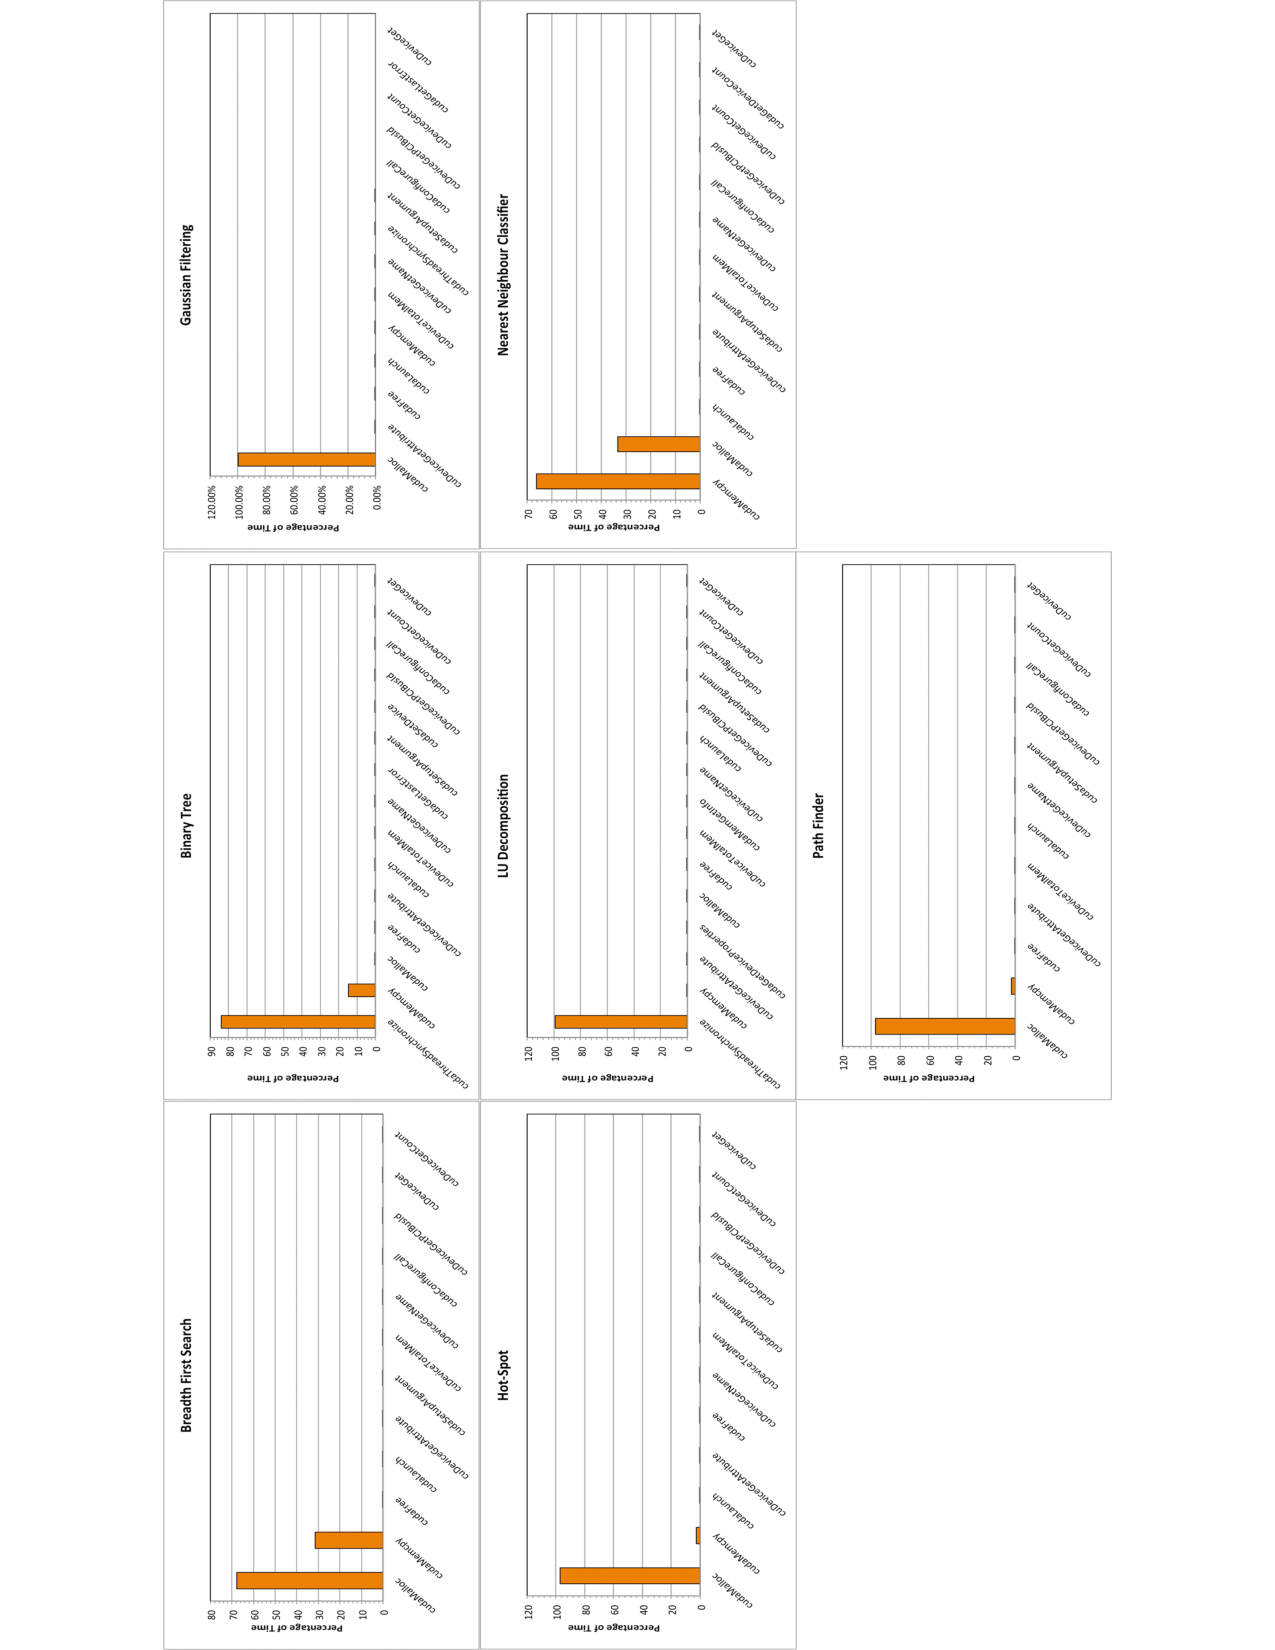
\includegraphics[scale=0.6]{../imgs/x630.pdf}
\caption{Time take for each API for seven test cases}
\label{Time take for each API for seven test cases}
\end{figure*}




\newpage
\section{Benchmarking using a GeForce GTX 650}
These tests have been performed using a GeForce GTX 650 and hardware platform 2 specified in Table \ref{table2}. The below figures depict the time take for each individual API call for all seven test cases.

\begin{figure*}[!h]
\centering
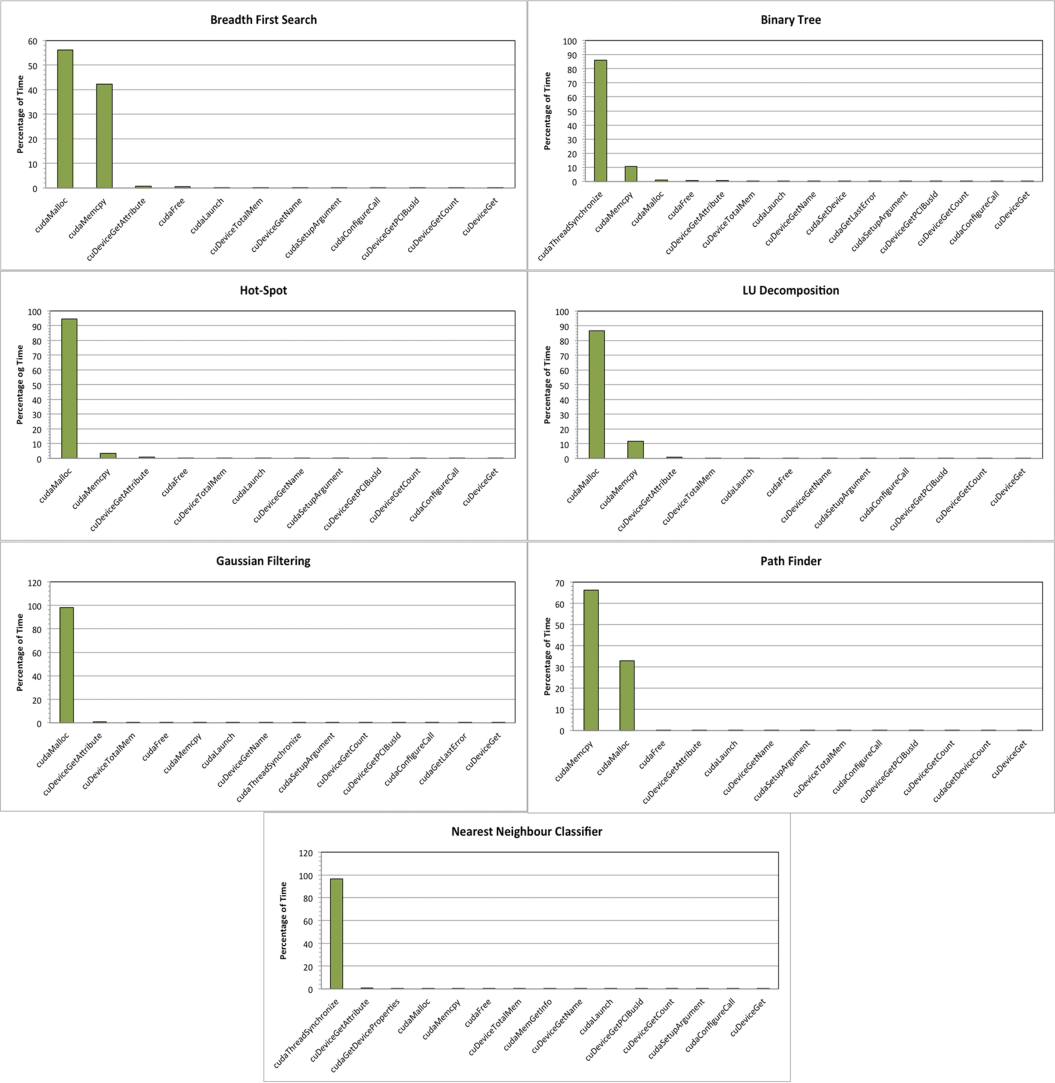
\includegraphics[scale=0.6]{../imgs/x650.pdf}
\caption{Time take for each API for seven test cases}
\label{Time take for each API for seven test cases}
\end{figure*}




\newpage
\section{Benchmarking using a Quadro 6000}
These tests have been performed using a Quadro 6000 and hardware platform 3 specified in the table in Table \ref{table2}. The below figures depict the time take for each individual API call for all seven test cases.

\begin{figure*}[!h]
\centering
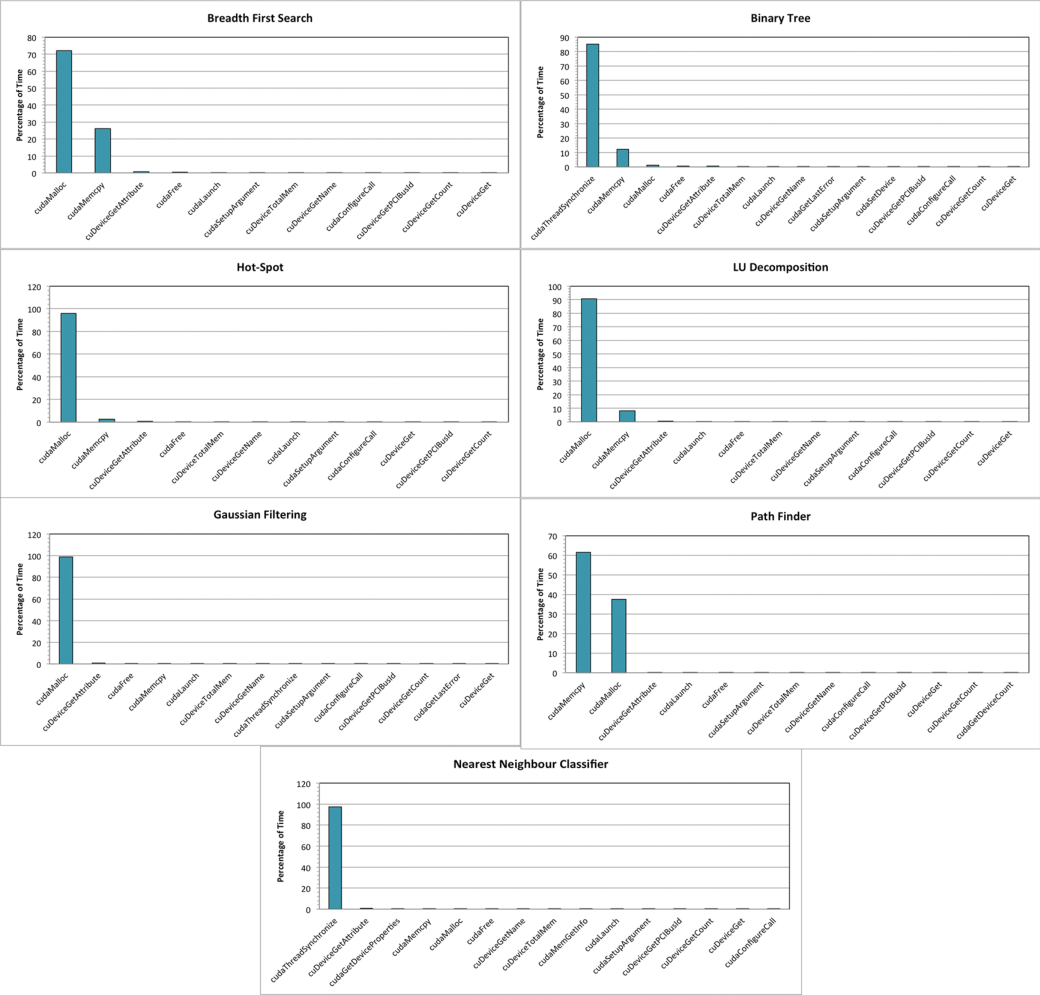
\includegraphics[scale=0.6]{../imgs/m6000.pdf}
\caption{Time take for each API for seven test cases}
\label{Time take for each API for seven test cases}
\end{figure*}






\newpage
\section{Results}

The below figures summarize all the results from all three different NVIDIA GPUs. 


\begin{figure*}[!h]
\centering
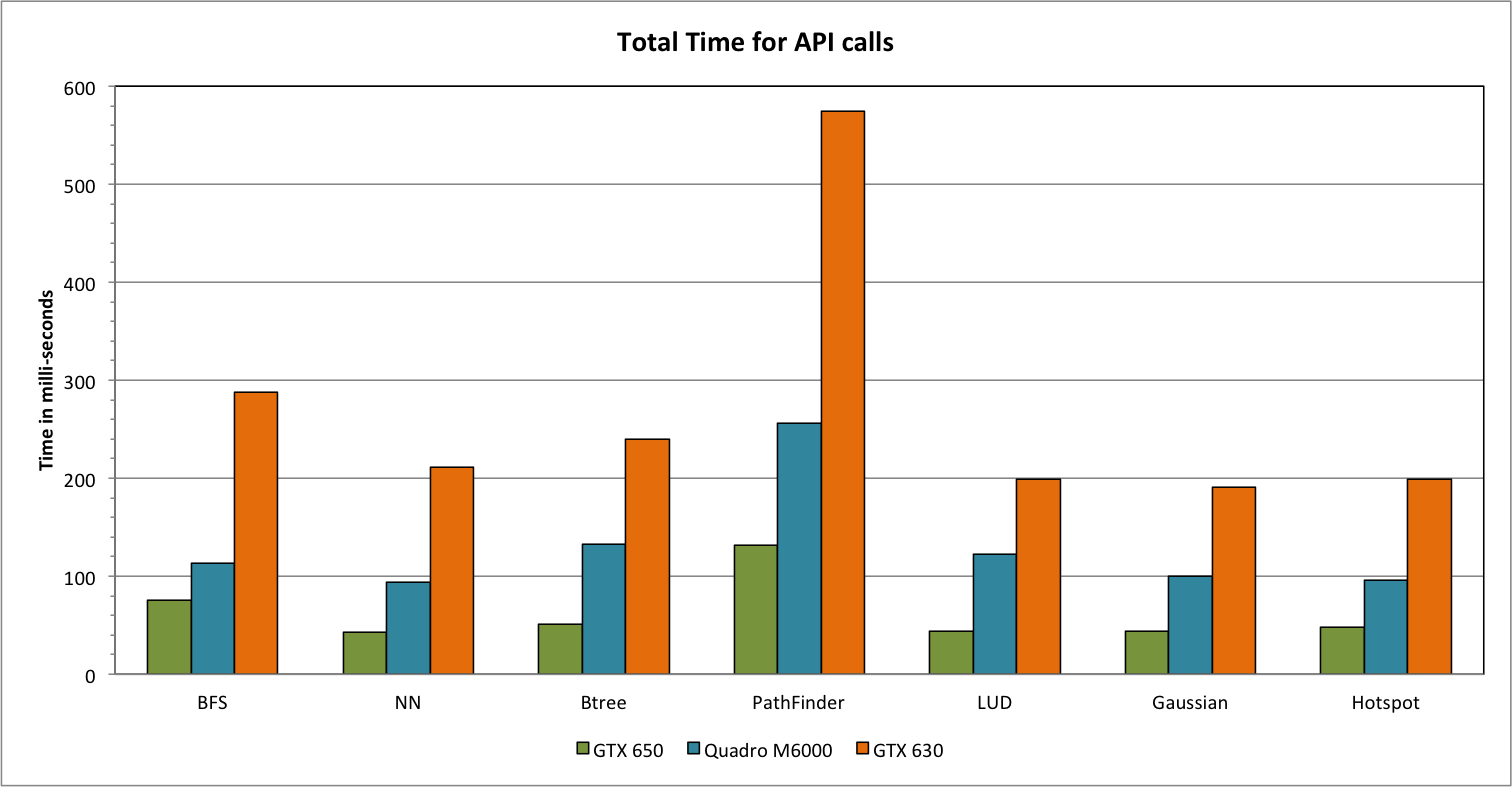
\includegraphics[width=0.95\textwidth,height=8cm]{../imgs/api_calls.png}
\caption{Total time for API calls for seven test cases}
\label{Total time for API calls for seven test cases}
\end{figure*}

\begin{figure*}[!h]
\centering
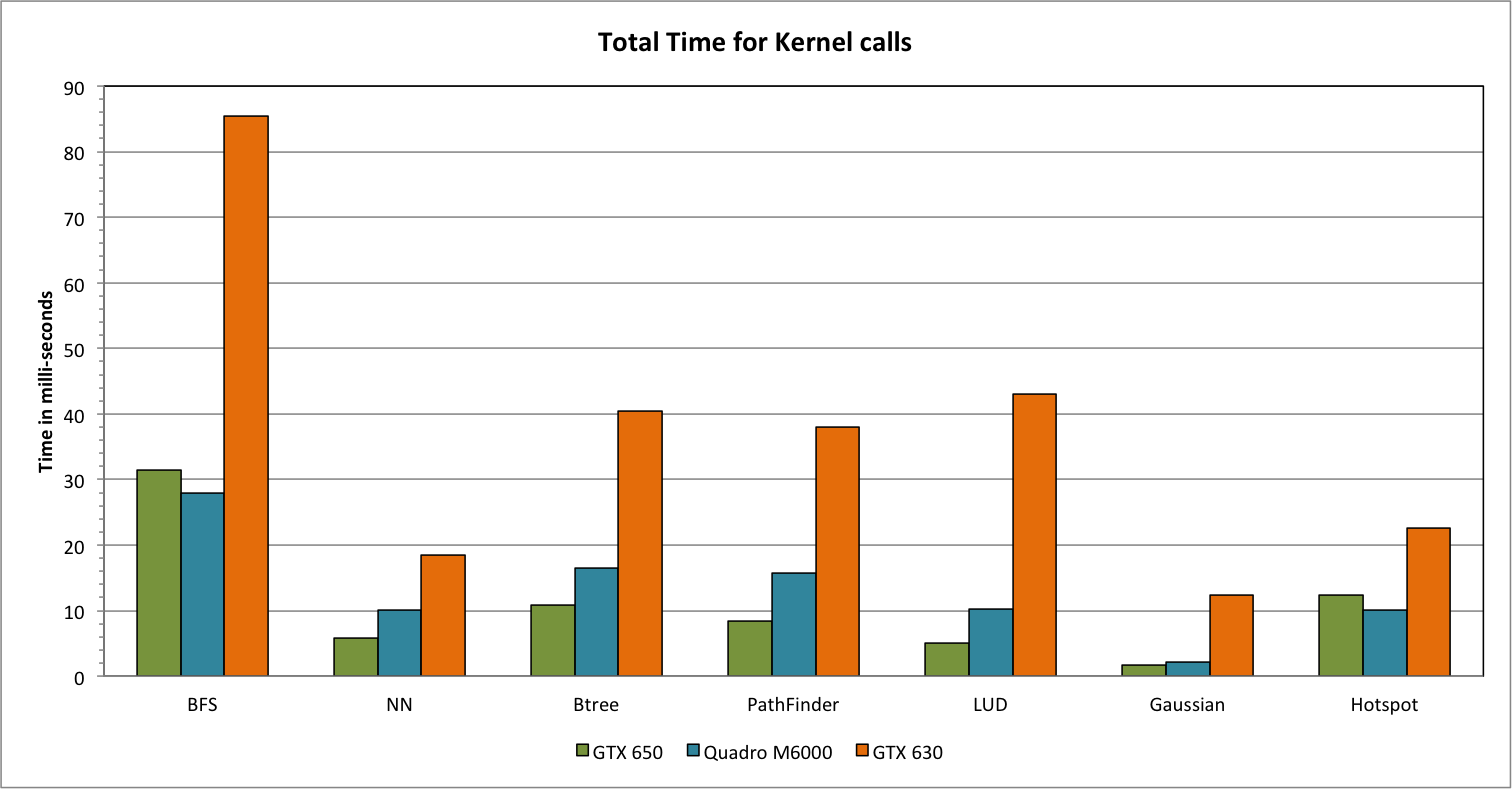
\includegraphics[width=0.95\textwidth,height=8cm]{../imgs/kernel_calls.png}
\caption{Total time for kernel calls for seven test cases}
\label{Total time for kernel calls for seven test cases }
\end{figure*}

\begin{figure*}[!h]
\centering
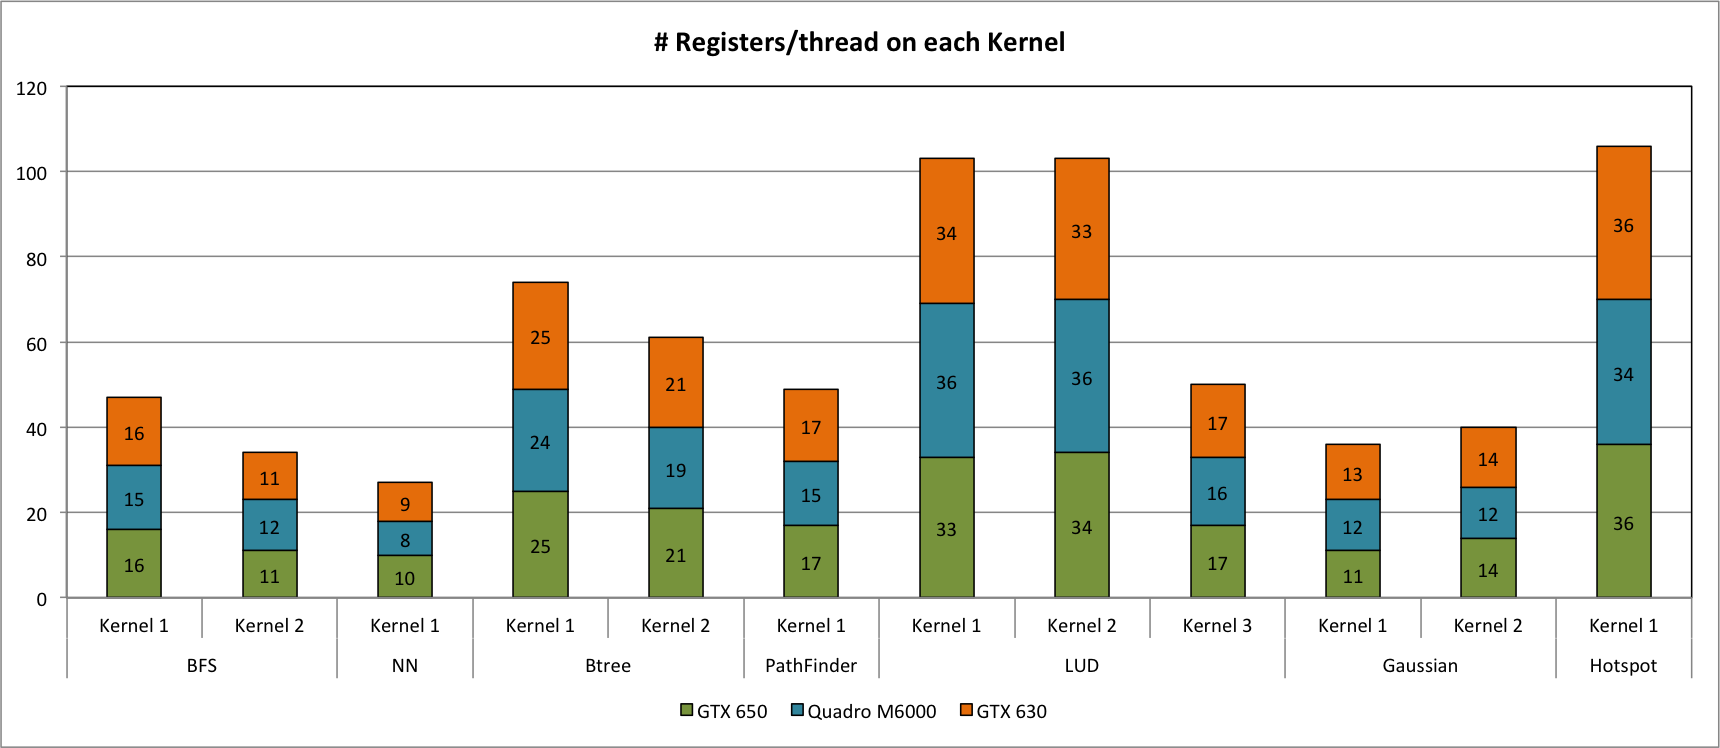
\includegraphics[width=0.95\textwidth,height=6cm]{../imgs/register_thread.png}
\caption{Number of registers per thread on each kernel for seven test cases}
\label{Number of registers per thread on each kernel for seven test cases}
\end{figure*}

\begin{figure*}[!h]
\centering
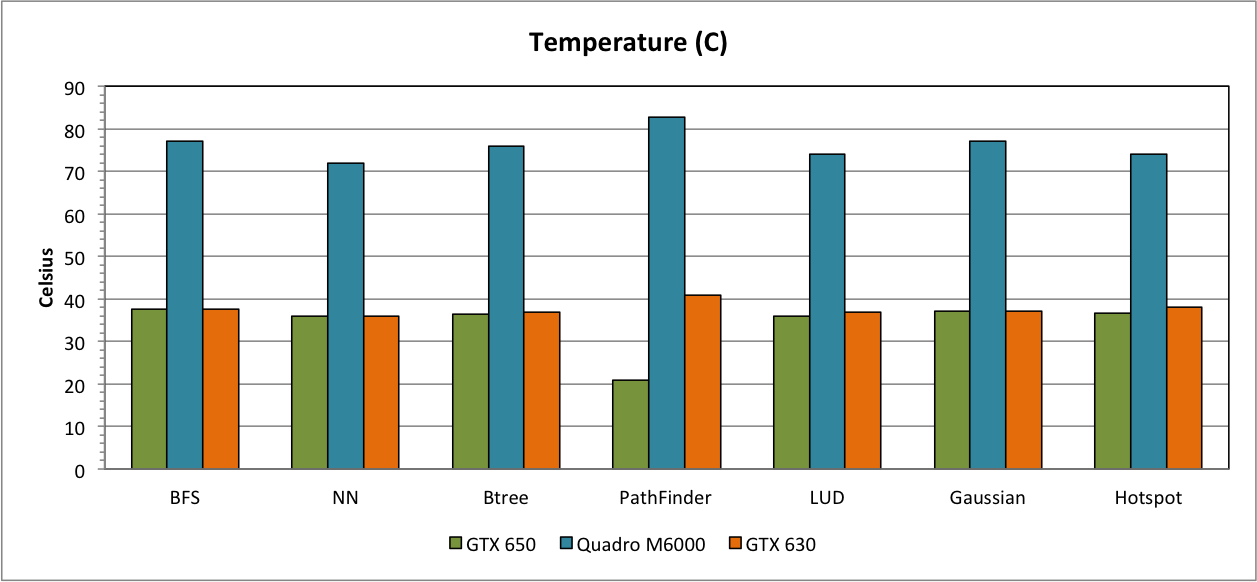
\includegraphics[width=0.95\textwidth,height=6cm]{../imgs/temp.png}
\caption{Temperature (C) for seven test cases}
\label{Temperature (C) for seven test cases}
\end{figure*}

\begin{figure*}[!h]
\centering
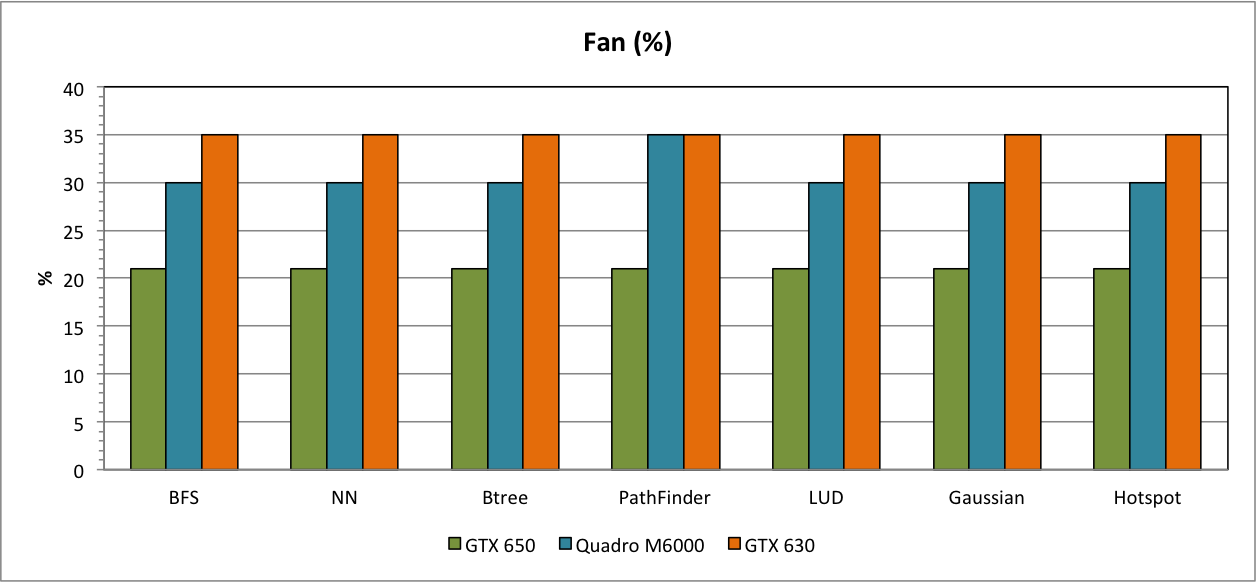
\includegraphics[width=0.95\textwidth,height=6cm]{../imgs/fan.png}
\caption{Fan spean for seven test cases}
\label{Fan spean for seven test cases}
\end{figure*}


\newpage
\section{Analysis}
.......


\newpage
\section{Conclusion}

Though the test cases ran for several seconds ..if they ran for minutes the differences will be even more profound


\end{document}
